\chapter{Návrh vylepšení systému}



\section{Možnosti odstranění omezení navržené gatewaye - závislost na znalosti typu koncových zařízení senzorové sítě}


%%%%%%%%%%%%%%%%%%%%%%%%%%%%%%%%%%%%%%%%%%%%%%%%%%%%%%
\section{Návrh gatewaye verze 2}
Pro lepší mechanické uspořádání byla navržena verze 2, kde je použit i jiný vývojový kit NUCLEO-L432KC s procesorem STM32L432KC, který je výkonnější.
Navíc je zde přidán externí stabilizátor, napěťový filtr, přepínačem volitelné impedanční zakončení sítě RS485 a proudové ochrany.

\begin{figure}[!h]
    \centering
    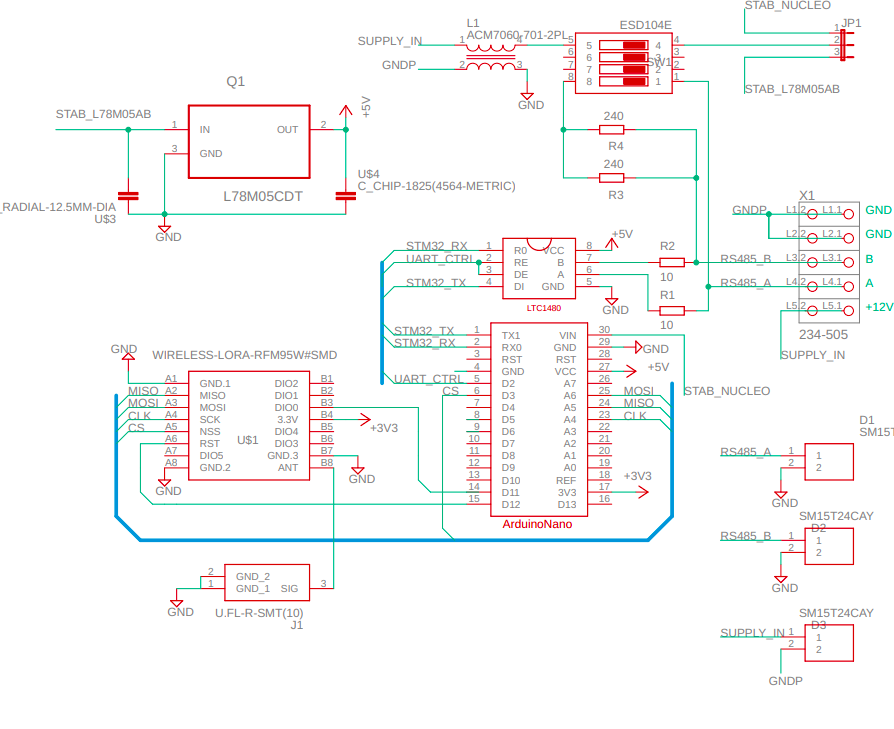
\includegraphics[width=1\textwidth]{minigateway_schema}
    \caption{Návrh WSN gatewaye verze 2 - schéma}
    \label{fig:minigateway_schema}
\end{figure}

\begin{figure}[!h]
    \centering
    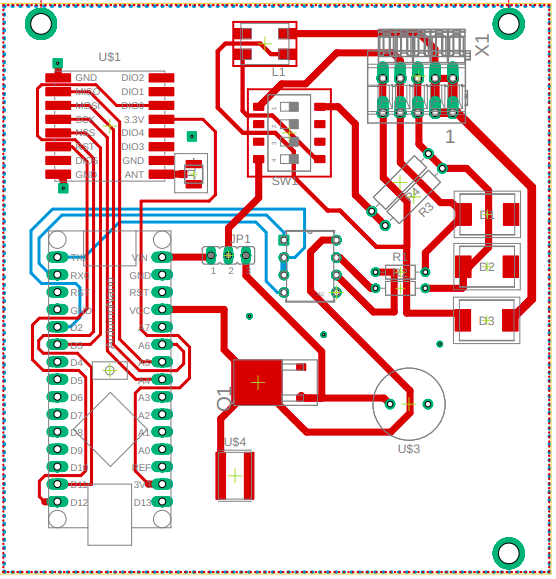
\includegraphics[width=0.7\textwidth]{minigateway_plosnak}
    \caption{Návrh WSN gatewaye verze 2 - plošný spoj}
    \label{fig:minigateway_plosnak}
\end{figure}




